\documentclass{beamer}
\usefonttheme[onlymath]{serif}
\usepackage{amsmath}
\usepackage{amsfonts}
\usepackage[export]{adjustbox}
\usepackage[utf8]{inputenc}
\usepackage{tikz} 
\usepackage{bm}
\usepackage{xkeyval}
\usepackage{todonotes}
\usepackage{mathtools}
\usepackage{graphicx}
\usepackage{caption}
\captionsetup[figure]{labelformat=empty}
\usepackage[ruled]{algorithm2e}
\newcommand{\D}{\mathbf{D}}
\newcommand{\Q}{\mathbf{Q}}
\DeclareMathOperator{\tr}{tr}
%Information to be included in the title page:
\usecolortheme{seahorse}
\title{Face Image Editing}
\author{Tianhao Wei \and Kangcheng Hou \and Shuqi Wang}
% \author[Short Name (U ABC)]{
%     \small
%     \texorpdfstring{
% \begin{columns}
%     \column{.25\linewidth}
%     \centering
%     Tianhao Wei \\ 3150104461
%     \column{.25\linewidth}
%     \centering
%     Kangcheng Hou \\ 3150102333
%     \column{.25\linewidth}
%     \centering
%     Shuqi Wang \\ 3150102288
%   \end{columns}
%   }
%   {Tianhao Wei, Kangcheng Hou, Shuqi Wang}
% }
\date{\today}

\begin{document}
    
\frame{\titlepage}

\begin{frame}{Introduction}
% 突出 face image editing 的重要性
\begin{itemize}
\item A large proportion of the images people upload is face image.
\item We want to develop a software that ease the process of editing facial image.
\end{itemize}
\end{frame}
\begin{frame}[allowframebreaks]{Applications}
\begin{columns}
\begin{column}{0.5\textwidth}\includegraphics[width=\textwidth]{./figs/expression-flow-img1.png}\end{column}
\begin{column}{0.5\textwidth}\includegraphics[width=\textwidth]{./figs/expression-flow-img2.png}\end{column}
\end{columns}
\framebreak
\begin{columns}
\begin{column}{0.5\textwidth}\includegraphics[width=\textwidth]{./figs/app1}\end{column}
\begin{column}{0.5\textwidth}\includegraphics[width=\textwidth]{./figs/app2}\end{column}
\end{columns}
\end{frame}
\begin{frame}{Agenda}
\begin{enumerate}
\item Generate a face
\item Fit a face model
\item Application: Expression Flow
\item Laplacian Surface Editing
\item Demo: Laplacian Surface Editing
\end{enumerate}
\end{frame}
\begin{frame}[allowframebreaks]{Generate a face}
% 我们可以是用常用的图像编辑软件去编辑一张人脸,例如photoshop,但是我们是需要简洁的方法来做这个事情,如果我们可以知道其中内部模型的构造,那么就会更好了。
% 首先我们要知道如何去生成一张人脸
% 大家使用的都是bilinear face model, 我们在网上找到了basel face model, 其提供的是下面这种,我们赶时间,就直接用下面这种了
Bilinear face model\cite{vlasic2005face}
$$\mathbf{f} = \mathcal{M} \times \mathbf{w}_{\text{id}}^\top \times \mathbf{w}_{\text{expr}}^\top$$
\includegraphics[width=\textwidth]{./figs/fig2.png}
Basel face model\cite{gerig2017morphable}
\begin{align*}
\mathbf{f} = \bar{\mathbf{f}} + \mathcal{M}_{\text{id}} \times \mathbf{w}_{\text{id}}^\top + \mathcal{M}_{\text{expr}}\times \mathbf{w}_{\text{expr}}^\top \\
\mathbf{w}_{\text{id}} \sim \mathcal{N}(0, \text{diag}(\sigma_{\text{id}}^{(1)}, \dots, \sigma_{\text{id}}^{(N_\text{id})}) \\ 
\mathbf{w}_{\text{expr}} \sim \mathcal{N}(0, \text{diag}(\sigma_{\text{expr}}^{(1)}, \dots, \sigma_{\text{expr}}^{(N_\text{expr})})
\end{align*}
% 这些基向量已经经过PCA处理,并且不同的基有不同的方差,服从高斯分布
% 我们看见的人脸还经过model view 矩阵变换,投影变换,最后变成现在这个样子
Under the assumption of weak perspective camera model, with scale $s$, rotation $\mathbf{R}$ and translation $\mathbf{t}$, we have 
$$\hat{\mathbf{f}} = s (\mathbf{R} \mathbf{f} + \mathbf{t})$$

\end{frame}

\begin{frame}{Fit a face model}
% 我们想要知道我们需要有怎么样的相机参数,以及什么样的人脸的identity和expression参数才能生成这样的人脸模型
Given an image and 2D face landmarks $\{l_1, \dots, l_{N_{\text{lm}}}\}$ from a off-the-shelf tracker\footnote{https://www.faceplusplus.com.cn/}. Solve the following optimization problem:
$$\min_{\mathbf{w}_{\text{id}}, \mathbf{w}_{\text{expr}}, s, \mathbf{R}, \mathbf{t}} \sum_{i=1}^{N_{\text{lm}}}||l_i - h_i||_2^2$$
where $\{h_1, \dots, h_{N_{\text{lm}}}\}$ is the corresponding points on 3d model.

% 但是没有closed form solution存在,不能弄一把least form solution 就可以了。使用coordinate descent.

\end{frame}


\begin{frame}{Coordinate Descent}
We alternate the optimization of $\color{red}{s, \mathbf{R}, \mathbf{t}}$ and $\color{blue}{\mathbf{w}_{\text{id}}, \mathbf{w}_{\text{expr}}}$.
$$\min_{\color{blue}{\mathbf{w}_{\text{id}}, \mathbf{w}_{\text{expr}}}, \color{red}{s, \mathbf{R}, \mathbf{t}}} \sum_{i=1}^{N_{\text{lm}}}||l_i - \color{red}{s}\color{black}(\color{red}\mathbf{R}\color{black}(\mathcal{M} \times [\color{blue}{\mathbf{w}_{\text{id}}, \mathbf{w}_{\text{expr}}} \color{black}]^\top)_i + \color{red}{\mathbf{t}} \color{black})||_2^2$$
\end{frame}


\begin{frame}{Algorithm: Fit a face model}
    \small
    \begin{algorithm}[H]
    \KwIn{facial landmarks $\{l_1, \dots, l_{N_{\text{lm}}}\}$ and PCA model}
    \KwOut{shape coefficients $\mathbf{w}$ and camera parameters $s,\mathbf{R},\mathbf{t}$}
    Set $\mathbf{w} = \mathbf{0}$\;
    \Repeat{$\mathbf{w}$ converges}{
        Set $\mathbf{f} = \bar{\mathbf{f}} + \mathcal{M} \times \mathbf{w}^\top$\;
        Find the camera parameters $s, \mathbf{R}, \mathbf{t}$ using $\mathbf{f}$ and $\{l_1, \dots, l_{N_{\text{lm}}}\}$\;
        Project all vertices of $\mathbf{f}$ onto the image plane: $\hat{\mathbf{f}} = s (\mathbf{R} \mathbf{f} + \mathbf{t})$\;
        Find the convex hull of $\hat{\mathbf{f}}$ as $\text{hull}(\hat{\mathbf{f}})$\;
        For contour landmarks $l_i$, find the correspondence\;
        Solve $\mathbf{w}$\;
    }   
    \caption{Fit face model to a single image}
    \end{algorithm}
    \end{frame}
% 首先是开始的点,我们会先设置一个初始的值,这时候我们看到是对的非常不好的
\begin{frame}[allowframebreaks]{Coordinate Descent}
\begin{columns}
\begin{column}{0.45\textwidth}\includegraphics[width=\textwidth]{./figs/iter0.png}\end{column}
\begin{column}{0.7\textwidth}\includegraphics[width=\textwidth]{./figs/cd0.pdf}\end{column}
\end{columns}
% 然后我们用"内点"估计相机参数,更新一下
\begin{columns}
\begin{column}{0.45\textwidth}\includegraphics[width=\textwidth]{./figs/iter1.png}\end{column}
\begin{column}{0.7\textwidth}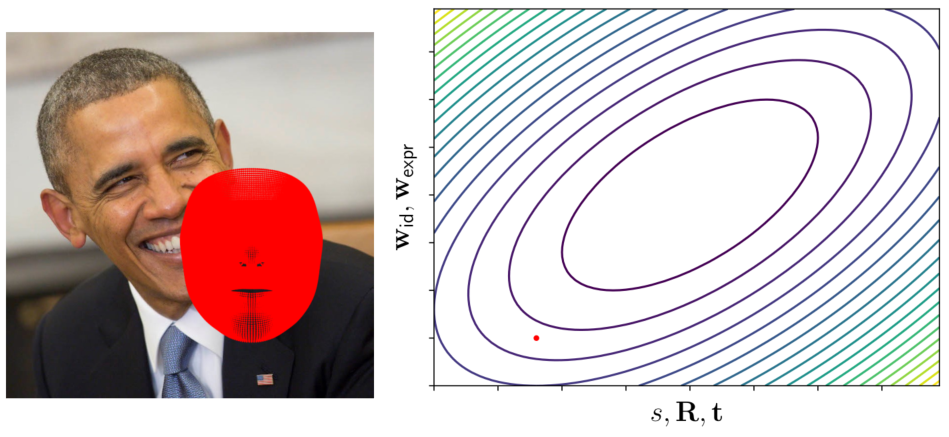
\includegraphics[width=\textwidth]{./figs/cd1.pdf}\end{column}
\end{columns}
% 然后我们找到convex hull, 找到correspondence
\begin{columns}
\begin{column}{0.45\textwidth}\includegraphics[width=\textwidth]{./figs/contour-match0.png}\end{column}
\begin{column}{0.7\textwidth}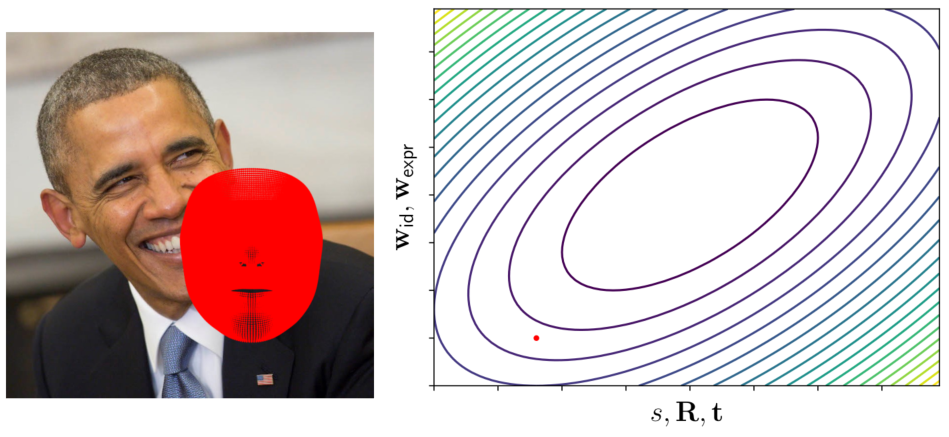
\includegraphics[width=\textwidth]{./figs/cd1.pdf}\end{column}
\end{columns}
% 然后我们根据这些correspondence 进行id_coef, exp_coef 的更新
\begin{columns}
\begin{column}{0.45\textwidth}\includegraphics[width=\textwidth]{./figs/iter2.png}\end{column}
\begin{column}{0.7\textwidth}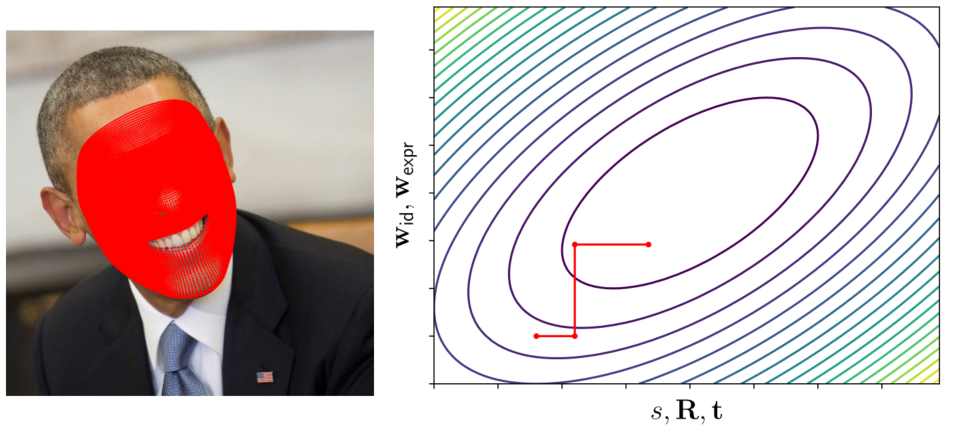
\includegraphics[width=\textwidth]{./figs/cd2.pdf}\end{column}
\end{columns}
% 然后我们再重复进行,估计相机参数
\begin{columns}
\begin{column}{0.45\textwidth}\includegraphics[width=\textwidth]{./figs/iter3.png}\end{column}
\begin{column}{0.7\textwidth}\includegraphics[width=\textwidth]{./figs/cd3.pdf}\end{column}
\end{columns}
% 找 convex hull
\begin{columns}
\begin{column}{0.45\textwidth}\includegraphics[width=\textwidth]{./figs/contour-match0.png}\end{column}
\begin{column}{0.7\textwidth}\includegraphics[width=\textwidth]{./figs/cd3.pdf}\end{column}
\end{columns}
% update id_coef, exp_coef
\begin{columns}
\begin{column}{0.45\textwidth}\includegraphics[width=\textwidth]{./figs/iter4.png}\end{column}
\begin{column}{0.7\textwidth}\includegraphics[width=\textwidth]{./figs/cd4.pdf}\end{column}
\end{columns}
\end{frame}

\begin{frame}{Estimation of Parameters}
\begin{itemize}
\item Estimation of $\mathbf{w}_{\text{id}}, \mathbf{w}_{\text{expr}}$ is a regularized least square.
\item Estimation of $s, \mathbf{R}, \mathbf{t}$ is achieved using POSIT algorithm.
\item See more in our report!
\end{itemize}
\end{frame}

% 我们现在可以来讲一个应用,我们经常会拍两张照片,一张表情效果比较好,另外一个表情效果不好,但是背景效果不错,我们如何去融合这两个图片?有了model fitting 以后我们就可以轻松地来弄了
\begin{frame}{Application: Expression Flow for 3D-Aware Face Component Transfer\cite{yang2011expression}}
    
\begin{columns}
\begin{column}{0.5\textwidth}\includegraphics[width=\textwidth]{./figs/expression-flow-img1.png}\end{column}
\begin{column}{0.5\textwidth}\includegraphics[width=\textwidth]{./figs/expression-flow-img2.png}\end{column}
\end{columns}
\end{frame}
\begin{frame}{Expression Flow Pipeline}
% \begin{figure}
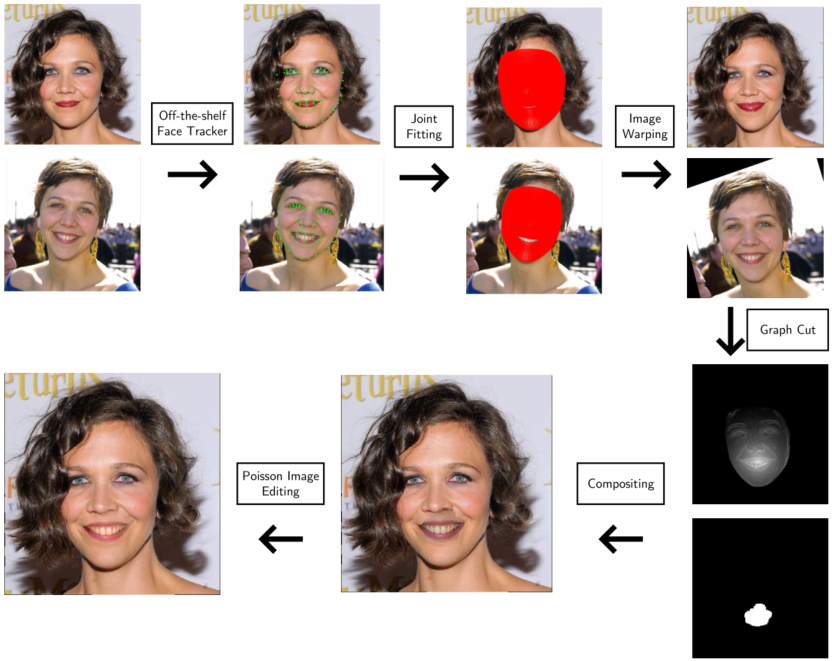
\includegraphics[width=\textwidth]{./figs/expression-flow-pipeline.pdf}
% \end{figure}
\end{frame}

\begin{frame}{More Results}
\begin{columns}[b]
\column{0.33\textwidth}\begin{figure}\includegraphics[width=\textwidth]{./figs/flow3/img1.png}\caption{Reference}\end{figure}
\column{0.33\textwidth}\begin{figure}\includegraphics[width=\textwidth]{./figs/flow3/img2.png}\caption{Target}\end{figure}
\column{0.33\textwidth}\begin{figure}\includegraphics[width=\textwidth]{./figs/flow3/blend_img.png}\caption{Result}\end{figure}
\end{columns}
\vspace{0pt}
\end{frame}

\begin{frame}{More Results}
\begin{columns}[b]
\column{0.33\textwidth}\begin{figure}\includegraphics[width=\textwidth]{./figs/flow2/img1.png}\caption{Reference}\end{figure}
\column{0.33\textwidth}\begin{figure}\includegraphics[width=\textwidth]{./figs/flow2/img2.png}\caption{Target}\end{figure}
\column{0.33\textwidth}\begin{figure}\includegraphics[width=\textwidth]{./figs/flow2/blend_img.png}\caption{Result}\end{figure}
\end{columns}
\vspace{0pt} 
\end{frame}

% 刚刚这种情况下,我们只能局限于已经存在的图片,那么我们能不能够对其进行一些编辑呢?我们首先来介绍laplacian mesh editing,比如说我们希望让一个mesh的鼻子提高一点,我们这时候不能去找一个新的图片来做这个事情,我们可以不可以按照我们想要的来编辑呢?
% 比如说,我们希望把一个mesh的鼻子拉长,那这种怎么做呢?这个问题就是我们有了一个约束,然后我们希望这个约束得到满足,而且保证尽可能光滑


\begin{frame}[allowframebreaks]{Laplacian Surface Editing}
Laplacian operator measures the flatness of the mesh:
$$\Delta f(\mathbf{x}) = \lim_{|B(\mathbf{x})| \rightarrow 0} \frac{1}{|B(\mathbf{x}))|} \int_{B(\mathbf{x})} f(\mathbf{z}) \;d\mathbf{z} - f(\mathbf{x})$$
Where $B(\mathbf{x})$ is an infinitesimal region around $\mathbf{x}$.
We want to the difference of mesh before and after deformation be small.  
\begin{align*}
\int_\Omega ||\Delta(\mathbf{x} - \hat{\mathbf{x}})||^2 \; d\mathbf{A} & \approx \text{tr}( \mathbf{D}^\top \mathbf{L}^\top \mathbf{M}^{-\top} \mathbf{M} \mathbf{M}^{-1} \mathbf{L}\mathbf{D})\\
&= \text{tr}(  \mathbf{D}^\top \underbrace{\mathbf{L}^\top \mathbf{M}^{-1} \mathbf{L}}_{\Q} \mathbf{D})
\end{align*}
where $\mathbf{D}, \mathbf{L}, \mathbf{M}$ is the difference of mesh, laplacian and the mass matrix respectively. 
$$
\min_{\D_\text{u}}
\tr \left((\D_\text{u}^\top \ \D_\text{h}^\top)
\left(\begin{array}{cc}
\Q_\text{u,u} & \Q_\text{u,h} \\
\Q_\text{h,u} & \Q_\text{h,h} 
\end{array}\right)
\left(\begin{array}{c}
  \D_\text{u} \\
  \D_\text{h}
\end{array}
\right)\right)
$$
$$
\min_{\D_\text{u}}
\tr\left(\D_\text{u}^\top \Q_\text{u,u} \D_\text{u} +
2 \D_\text{u}^\top \Q_\text{u,h} \D_\text{h} + 
\underbrace{\D_\text{h}^\top \Q_\text{h,h}
\D_\text{h}}_\text{constant}\right)
$$
$$
\min_{\D_\text{u}} 
\tr\left(
\D_\text{u}^\top \Q_\text{u,u} \D_\text{u} +
2 \D_\text{u}^\top \Q_\text{u,h} \D_\text{h})
\right)
$$
Set the gradient to zero
$$2 \Q_\text{u,u} \D_\text{u} + 2 \Q_\text{u,h} \D_\text{h} = 0 \rightarrow \D_\text{u} = \Q_\text{u,u}^{-1} \Q_\text{u,h} \D_\text{h}$$
Minimization w.r.t to the unconstrained points gives us the solution.
\end{frame}
\begin{frame}
\begin{center}
\Huge Demo: \\Laplacian Surface Editing
\end{center}
\end{frame}
% 我们现在就可以修改mesh啦,我们来看一看效果,可以让一个人的笑容变得更大,可以改变他嘴巴的大小,TODO: 明天随便找几个图片做一下效果就好了。我们本来想做一个旋转的,但是现在的效果已经够好了,所以就没有继续做下去。ARAP的效果并不好,可以大概展示一下。
\begin{frame}{Results}
    \includegraphics[width=\textwidth]{./figs/laplacian.pdf}
\end{frame}


\begin{frame}{Summary}
What have we implemented?
\begin{itemize}
\item Single/Joint Face fitting \cite{yang2011expression}
\item Laplacian Surface Editing \cite{sorkine2004laplacian}
\item Poisson Image Editing \cite{perez2003poisson}
\item Formulate our problem into graph cut\cite{yang2011expression} and solve it using GCO library \cite{boykov2004experimental}
\item ARAP shape manipulation \cite{igarashi2005rigid}
\item \textbf{Combine the above all together}
\end{itemize}
% Personalized Face Editing is a part of Computer Graphics 2.0!\cite{zhou2017computer}
\end{frame}

\begin{frame}[allowframebreaks]{References}
\bibliographystyle{apalike}
\setbeamertemplate{bibliography item}[article]
\bibliography{ref}
\end{frame}

\begin{frame}
\begin{center}
\Huge Thanks!
\end{center}
\end{frame}
\end{document}